\documentclass[10pt]{article}
\usepackage[utf8]{inputenc}
\usepackage[english]{babel}
\usepackage[margin=1in]{geometry}
% \newcommand\hmmax{0}
% \newcommand\bmmax{0}

% % % Fonts% %
   \usepackage[T1]{fontenc}
   % \usepackage{textcomp}
   % \usepackage{newtxtext}
   % \renewcommand\rmdefault{Pym} %\usepackage{mathptmx} %\usepackage{times}
   \usepackage[complete, subscriptcorrection, slantedGreek, mtpfrak, mtpbbi, mtpcal]{mtpro2}
   \usepackage{bm}% Access to bold math symbols
   % \usepackage[onlytext]{MinionPro}
   \usepackage[no-math]{fontspec}
   \defaultfontfeatures{Ligatures=TeX,Numbers={Proportional}}
   \newfontfeature{Microtype}{protrusion=default;expansion=default;}
   \setmainfont[Ligatures=TeX]{TimesNRMTPro}
   \setsansfont[Scale=MatchLowercase,Ligatures=TeX]{Myriad Pro}
   \setmonofont[Scale=0.8]{mononoki}

   \newfontfamily{\unifont}[Ligatures=TeX]{Menlo}

   % \usepackage{selnolig}% For suppressing certain typographic ligatures automatically
   \usepackage{microtype}
% % % % % % % % %
\usepackage{amsthm}         % (in part) For the defined environments
\usepackage{mathtools}      % Improves  on amsmaths/mtpro2
\usepackage{bbding}         % For hand pointers, etc.

% % The bibliography % % %
\usepackage[backend=biber,
            style=authoryear-comp,
            citestyle=authoryear-comp,
            backref=false,
            hyperref=true,
            url=false,
            isbn=false,
           ]{biblatex}
% % \renewcommand*{\bibfont}{\small}
\DeclareFieldFormat{postnote}{#1}
\DeclareFieldFormat{multipostnote}{#1}
% \setlength\bibitemsep{1.5\itemsep}
\addbibresource{ling245.bib}

% \newcommand{\seccite}[1]{\citeauthor{#1}, \citetitle{#1}, \citeyear{#1}}
% % % % % % % % % % % % % % %

% % % % % % % % % % % % % % % % % % % % % % % % % % % % % %

% % % Custom Commands % % %
% \newcommand{\subfor}[2]{[\sfrac{#1}{#2}]}
\usepackage{xfrac,nicefrac} % For \sfrac{i}{j} and for nicer fractions
\newcommand{\sem}[1]{\ensuremath{[\kern-.5mm[{#1}]\kern-.5mm]}}
% % % % % % % % % % % % % %

\usepackage[inline]{enumitem}
% \setlist[enumerate]{itemsep=.03125em}
  \setlist[itemize]{noitemsep}
  \setlist[description]{noitemsep,style=unboxed,leftmargin=.5cm,font=\normalfont\space}
  \setlist[enumerate]{noitemsep}
% % %

% % For Figures % % %
\usepackage{tikz} % For drawings
\usepackage{graphicx}
\usepackage{pgfplots}
% \pgfplotsset{compat=1.15}
\usepackage{wrapfig}
\usepackage{float} % For correctly placed floats
\usepackage{subcaption}
% \captionsetup{compatibility=false}
% % % % % % % % % % %

% For plots


% \usepackage{graphicx}

% % % Misc packages % % %

% \usepackage{refcheck} % Can be used for checking references
% \usepackage{lineno}   % For line numbers
\usepackage{multicol} % For multiple columns
% \usepackage{mathrsfs} % For elegant Latin math letters
% \usepackage{hyphenat} % For \hyp{} hyphenation command, and general hyphenation stuff
% \usepackage{titling} % for multiple titles
% % % % % % % % % % % % %

\usepackage{chngcntr}
\counterwithout{paragraph}{subsubsection}
\renewcommand{\theparagraph}{\arabic{paragraph}.}
\setcounter{secnumdepth}{4}
\usepackage{titlesec}
% \titleformat{\paragraph}[runin]{\normalfont}{\indent}{\wordsep}{}
% \titlespacing{\paragraph}{0pt}{3.25ex plus 1ex minus .2ex}{5\wordsep}
% \titleformat{\paragraph}[runin]{\normalfont}{}{\wordsep}{}
% \titlespacing{\paragraph}{0pt}{1ex plus .2ex minus .2ex}{0pt}
\titleformat{\paragraph}[hang]{\em}{}{0em}{}
\titlespacing{\paragraph}{0pt}{3.25ex plus 1ex minus .2ex}{5\wordsep}

\usepackage[export]{adjustbox}

\usepackage[hidelinks,breaklinks]{hyperref}



\title{Ling 245 Class Project Paper}
\author{Benjamin Sparkes}
% \date{}

\begin{document}

% % Begin data
\pgfplotstableread[row sep=\\, col sep=&]{
primeCategory  & meanPercent & meanPlusSEPercent& meanMinusSEPercent&  rawMean  &  rawSD   & rawSE & rawMeanPlusSE & rawMeanMinusSE & percentError \\
strongNUM4NUM4 &  0.6767956 & 0.7208479 & 0.6327433 &  2.634409 & 1.653619 & 0.1714723 & 2.805881 & 2.462936 & 0.0511447 \\
weakNUM4NUM4 &  0.5675553 & 0.6129002 & 0.5222103 &  2.184783 & 1.683334 & 0.1745536 & 2.359336 & 2.010229 & 0.0526454 \\
}\NUMNUMData


\pgfplotstableread[row sep=\\, col sep=&]{
primeCategory  & meanPercent & meanPlusSEPercent& meanMinusSEPercent&  rawMean  &  rawSD   & rawSE & rawMeanPlusSE & rawMeanMinusSE & percentError \\
strongNUM4SOME &  0.5762712 & 0.6226379 & 0.5299045 &  2.193548 & 1.702032 & 0.1764925 & 2.370041 & 2.017056 & 0.0538317 \\
weakNUM4SOME &  0.5833029 & 0.6305801 & 0.5360257 &  2.239130 & 1.750162 & 0.1814834 & 2.420614 & 2.057647 & 0.0548888 \\
}\NUMSOMEData

\pgfplotstableread[row sep=\\, col sep=&]{
primeCategory  & meanPercent& meanPlusSEPercent& meanMinusSEPercent&  rawMean  &  rawSD   & rawSE & rawMeanPlusSE & rawMeanMinusSE & percentError \\
strongSOMENUM4 &  0.7414502 & 0.7903533 & 0.6925471 &  2.511364 & 1.597371 & 0.1656396 & 2.677003 & 2.345724 & 0.0567766 \\
weakSOMENUM4 &  0.6498584 & 0.6947576 & 0.6049591 &  2.466667 & 1.643510 & 0.1704240 & 2.637091 & 2.296243 & 0.052128 \\
}\SOMENUMData

\pgfplotstableread[row sep=\\, col sep=&]{
primeCategory  & meanPercent& meanPlusSEPercent& meanMinusSEPercent&  rawMean  &  rawSD   & rawSE & rawMeanPlusSE & rawMeanMinusSE & percentError \\
strongSOMESOME &  0.6966165 & 0.7497500 & 0.6434830 &  2.329545 & 1.713514 & 0.1776831 & 2.507229 & 2.151862 & 0.061688 \\
  weakSOMESOME &  0.4780198 & 0.5732846 & 0.4780198 &  1.978261 & 1.728737 & 0.1792617 & 2.157523 & 1.798999 & 0.1106024 \\
}\SOMESOMEData
% % End data

\maketitle


\begin{abstract}
  Partial replication of Experiment 1 from \textcite{Bott:2016aa}.
  Main results are:
  \begin{enumerate*}[label=\alph*)]
  \item Replication of priming effects in general,
  \item failure to replicate between-category priming effect,
  \item replication of within-category priming effect,
  \item replication of no significant effects when splitting the data in half,
  \item replication of no significant effect in between-category priming with respect to the prime and target categories.
  \end{enumerate*}
  Main theoretical result: less support for shared reasoning processes between distinct instances of enrichment via alternatives.
\end{abstract}

\begin{multicols}{2}

% \section*{Things to Note}
% \label{sec:things-note}

% Need a decent number of observations from each individual on each trial for the analysis \citeauthor{Bott:2016aa} perform to work.
% Here, `decent number' means that we need at least one primeStrength and (WithCat/BetCat) trial with correct prime choices, else there are going to be fewer observations than random effects.

\section{Introduction}
\label{sec:introduction}

The core question of \textcite{Bott:2016aa} is whether or not there are shared reasoning processes which apply to distinct instances of enrichment via alternatives, or whether each category of enrichment has its on specialised process.
(\citeyear[118]{Bott:2016aa})
One may worry that this begs the question with respect to what kind of explanation one should give to pragmatic reasoning of the kind considered by \citeauthor{Bott:2016aa} in favour of enrichment via alternatives.
There are two items to note in this respect.
First, assuming that an explanation is correct is not quite the same as begging the question.
So long as we, or \citeauthor{Bott:2016aa}, are not attempting to support enrichment via alternatives as an explanation for (certain cases of) pragmatic reasoning, there's no worry in assuming that it's correct.
Second, \citeauthor{Bott:2016aa}, indeed, are not attempting to support enrichment via alternatives as an explanation for (certain cases of) pragmatic reasoning.
This may not appear to be consistent with statements such as:
`Our approach was to test whether enrichments can be primed across expressions.' (\citeyear[118]{Bott:2016aa}).
This may suggests that \citeauthor{Bott:2016aa} are interested in whether priming can occur at all, but when this is followed by:
`If different sorts of enrichments can prime each other, there must be an abstract mechanism that is shared between them.
By testing which enrichments prime each other and which don’t, we can specify what the common mechanism might be.' (\citeyear[118]{Bott:2016aa})
It should be clear that \citeauthor{Bott:2016aa} are interested in whether priming can occur at all \emph{given} a prior assumption of enrichment via alternatives.

The question of whether or not there are shared reasoning processes which apply to distinct instances of enrichment via alternatives, or whether each category of enrichment has its on specialised process has a nice cognitive feel.
For, it would seem that there's some positive upshot whichever way the data points.
If there is cross-category enrichment, then there is a need to posit shared reasonig processes.
And, if there is no cross-category enrichment, then one should posit distinct reasoning processes.
While the question has a nice cognitive feel given these resolutions, it is important to note that each of these carries a presupposition that the data can/should/will support one of these resolutions.
However, (and as we shall see) there is no guarantee that the data will be so clean.

\citeauthor{Bott:2016aa} ran three experiments, in which participants are presented with trials consisting of a setence and two picutures, and are asked to select the picture which best reflects the sentence.
We'll go into the details below, as for now the relevant detail is that trials are split into \emph{prime} and \emph{response}, and every response trial is preceeded by two prime trials which are used to ensure the participant considers certain alternatives.
For the two pictures in the response trial, one picture is consistent with the semantic content of the sentence, and the other contains the words `Better Picture?', which the participants were instructed to click if they felt the the other picture did not sufficiently capture the sentence meaning.
This allows us to state the basic linking hypothesis, which is that prior trials will effect how participants evaluate sentences, and that in response trials participants click on `Better Picture?' if they process the setence pragmatically, and the semantically adequate picture otherwise.

\citeauthor{Bott:2016aa} do not make predictions regarding the results of the experiment.
Instead, their core interest is in how the question noted above should be resolved.
However, they do note that `[i]f enrichment can be primed at all, we would expect within-category priming' and that `[i]f the \emph{numbers}, \emph{some} and \emph{ad hoc} EVAs share enrichment mechanisms we would expect them to prime each other, so that a strong some prime, for example, leads to a greater proportion of strong number responses.'
(\citeyear[122]{Bott:2016aa})
And, from the results of \citeauthor{Bott:2016aa}'s experiment, one should expect to see a significant effect of priming, both within and between categories.

This paper contains the results of a (partial) replication of Experiment 1 of \textcite{Bott:2016aa}.
The replication is partial for two reasons:
\begin{enumerate*}[label=\arabic*)]
\item the replication ran with half the number of participants compared with \citeauthor{Bott:2016aa}'s original experiment (100 and 200 participants, respectively), and
\item the replication contained only two enrichment categories, as opposed to three in the original.
\end{enumerate*}
The basis for both modifications was straightforward cost considerations, and by uncommenting a few lines of code (and fixing any bugs that this may cause) allows for the full experiment to be run.
We will discuss the second aspect of this modification in detail after reviewing \citeauthor{Bott:2016aa}'s paper.

The code for the experiment, data collected, analysis scripts, and other relevant resources can be found at \url{https://github.com/bsparkes/bottchemla2016}\nolinebreak
\footnote{Though \url{https://gitlab.com/bsparkes/bottchemla2016} is more likely to stick around.}\nolinebreak
, and one can experience the experiment at \url{https://bsparkes.github.io/bottchemla2016/experiment/html/bottchemla2016.html}.

The experiment was registered with OSF (\url{https://osf.io/5bnmr/register/5771ca429ad5a1020de2872e}).
Though, due to forgetfulness this was not strictly a \emph{pre}registration as the experiment had been initialised earlier the same day.
Still, as the analysis of the experiment will follow that of \citeauthor{Bott:2016aa}, there isn't much room for funny business.





\section{The Experiment}
\label{sec:experiment}

\begin{figure*}[ht]
 \centering
  \begin{tikzpicture}[scale=1]
    \draw (-7,0) -- (-2,0);
    \node[text width=6cm] at (-2,5) {\emph{Prime}};
    \node[text width=6cm] at (7,5) {\emph{Target}};
    \node[text width=6cm] at (-5.75,2.125) {\emph{Strong}};
    \node[text width=6cm] at (-5.75,-2.375) {\emph{Weak}};
    \node[text width=6cm] at (-3.875,4) {\textsf{Some of the symbols are squares}};
    \node[inner sep=0pt] (p1L) at (-6,2) {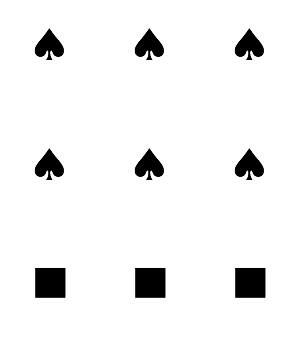
\includegraphics[width=.15\linewidth, frame]{images/p1LSpquares.png}};
    \node[inner sep=0pt] (p1R) at (-3,2) {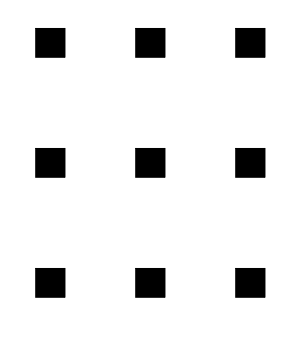
\includegraphics[width=.15\linewidth, frame]{images/p1RSquares.png}};
    \node[text width=6cm] at (-3.6,-.5) {\textsf{Some of the symbols are stars}};
    \node[inner sep=0pt] (p2L) at (-6,-2.5) {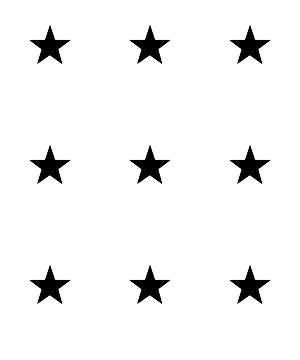
\includegraphics[width=.15\linewidth, frame]{images/p2LStars.png}};
    \node[inner sep=0pt] (p2R) at (-3,-2.5) {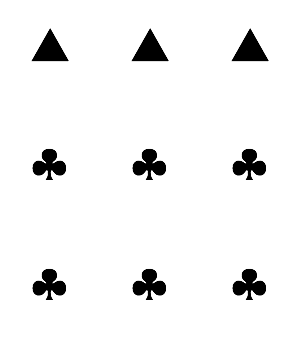
\includegraphics[width=.15\linewidth, frame]{images/p2RStars.png}};
    \node[text width=6cm] at (5.375,2) {\textsf{Four of the symbols are hearts}};
    \node[inner sep=0pt] (rL) at (3,0) {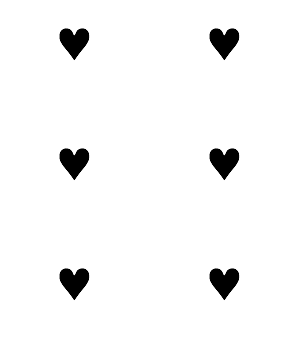
\includegraphics[width=.15\linewidth, frame]{images/responseFourH.png}};
    \node[inner sep=0pt] (rR) at (6,0) {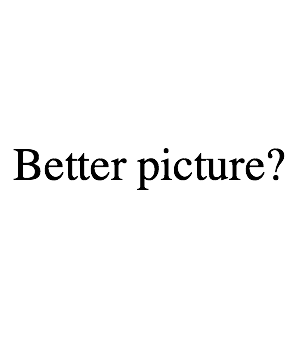
\includegraphics[width=.15\linewidth, frame]{images/bp.png}};
    \draw[->] (-1,2) -- (.75,1);
    \draw[->] (-1,-2) -- (.75,-1);
  \end{tikzpicture}
  \caption{\emph{Example stimuli for the replication.} Participants see two instances of a prime type followed by a target.
    The prime (left) consists of a sentence and two pictures, and the target (right) consists of one picture containing symbols and a `Better Picture?' option.
    Here, the schema for a cross category triplet is shown, when the prime is taken from the \emph{some} category, and the prime from the \emph{number}4 category.
    The symbols used were generated randomly, and the outlines for each picture had curved corners which I was too lazy to reproduce in tikz.
  }
  \label{fig:excards}
\end{figure*}

\subsection{Method}
\label{sec:method}


\begin{figure*}[ht]
\begin{subfigure}[]{.25\textwidth}
  \begin{tikzpicture}
    \begin{axis}[
      align =center,
      title = {Num4 \\ Num4},
      width=\textwidth,
      height=10cm,
      ybar=2*\pgflinewidth,
      enlarge x limits=1,
      bar width=25pt,
      symbolic x coords={strongNUM4NUM4, weakNUM4NUM4},
      xticklabels = {Strong, Weak},
      xtick={strongNUM4NUM4, weakNUM4NUM4},
      grid=major,
      ymax=1,
      ymin=0,
      enlarge x limits=.75,
      ]
      \addplot+[error bars/.cd,y dir=both,y explicit] table[x=primeCategory,y=meanPercent, y error=percentError]{\NUMNUMData};
    \end{axis}
  \end{tikzpicture}
\end{subfigure}%\hspace{2pt}
\begin{subfigure}[]{.25\textwidth}
  \begin{tikzpicture}
    \begin{axis}[
      align =center,
      title = {Num4 \\ Some},
      width=\textwidth,
      height=10cm,
      ybar=2*\pgflinewidth,
      enlarge x limits=1,
      bar width=25pt,
      symbolic x coords={strongNUM4SOME, weakNUM4SOME},
      xticklabels = {Strong, Weak},
      xtick={strongNUM4SOME, weakNUM4SOME},
      grid=major,
      ymax=1,
      ymin=0,
      yticklabels=\empty, % That's the trick
      enlarge x limits=.75,
      ]
      \addplot+[error bars/.cd,y dir=both,y explicit] table[x=primeCategory,y=meanPercent, y error=percentError]{\NUMSOMEData};
    \end{axis}
  \end{tikzpicture}
\end{subfigure}%\hspace{2pt}
\begin{subfigure}[]{.25\textwidth}
  \begin{tikzpicture}
    \begin{axis}[
      align =center,
      title = {Some \\ Num4},
      width=\textwidth,
      height=10cm,
      ybar=2*\pgflinewidth,
      enlarge x limits=1,
      bar width=25pt,
      symbolic x coords={strongSOMENUM4, weakSOMENUM4},
      xticklabels = {Strong, Weak},
      xtick={strongSOMENUM4, weakSOMENUM4},
      grid=major,
      ymax=1,
      ymin=0,
      yticklabels=\empty, % That's the trick
      enlarge x limits=.75,
      ]
      \addplot+[error bars/.cd,y dir=both,y explicit] table[x=primeCategory,y=meanPercent, y error=percentError]{\SOMENUMData};
    \end{axis}
  \end{tikzpicture}
\end{subfigure}%\hspace{pt}
\begin{subfigure}[]{.25\textwidth}
  \begin{tikzpicture}
    \begin{axis}[
      align =center,
      title = {Some \\ Some},
      width=\textwidth,
      height=10cm,
      ybar=2*\pgflinewidth,
      enlarge x limits=1,
      bar width=25pt,
      symbolic x coords={strongSOMESOME, weakSOMESOME},
      xticklabels = {Strong, Weak},
      xtick=data,
      grid=major,
      ymax=1,
      ymin=0,
      yticklabels=\empty, % That's the trick
      enlarge x limits=.75,
      ]
      \addplot+[error bars/.cd,y dir=both,y explicit] table[x=primeCategory,y=meanPercent, y error=percentError]{\SOMESOMEData};
    \end{axis}
  \end{tikzpicture}
\end{subfigure}
\caption{\emph{Replication results}. Priming is shown by the difference between the strong and weak bars for each panel. The label at the top of each panel shows the prime and response types.
  For example, the third panel, labelled `Some, Num4' corresponds to priming with \emph{some} and a \emph{number}4 response.\protect\footnotemark
  \space It is unclear what the error bars for the corresponding panels are for \citeauthor{Bott:2016aa}, here the error bars correspond to 90\% confidence intervals.}
  \label{tab:barresults}
\end{figure*}
\footnotetext{Unlike \citeauthor{Bott:2016aa}'s results for the experiment 1, we keep the between category priming groups distinct (see \textcite[Fig.\ 2, 122]{Bott:2016aa}).
  However, \citeauthor{Bott:2016aa} also present distinct results for \emph{some} and \emph{number}4 respones when compiling the results from all three of their experiments, and so the panels may be compared to these (see \textcite[Fig.\ 6, 133]{Bott:2016aa}).}


\paragraph{Materials}

The experiment consistent of trails, where each involved two pictures presented below a sentence.
Participants were asked to select one of the two pictures which best reflects the sentence.
The sentence was constructed using one of two frames:
\begin{enumerate*}[label=(\roman*)]
\item Some of the symbols are [symbol]
\item There are four [symbol]
\end{enumerate*}
\citeauthor{Bott:2016aa} included a third frame:
\begin{enumerate*}[label=(\roman*), resume]
\item There is a [symbol].
\end{enumerate*}
As mentioned in the introduction, this frame was excluded for cost considerations.
We shall keep track of the differences to the experiment which follow from using two frames as opposed to three in this section, and engage in a broader discussion in the Discussion portion of this paper.

The symbols were one of diamonds, clubs, ticks, spades, hearts, squares, stars, circles, notes, or triangles.\nolinebreak
\footnote{The following unicode sybomls were used: {\space\unifont ♦\space} \mbox{ }  {\space\unifont ♣\space} \mbox{ } {\space\unifont ✓\space} \mbox{ } {\space\unifont ♠\space} \mbox{ } {\space\unifont ♥\space} \mbox{ } {\space\unifont ◼\space} \mbox{ } {\space\unifont ★\space} \mbox{ } {\space\unifont ●\space} \mbox{ } {\space\unifont ♩\space} \mbox{ } {\space\unifont ▲}.
  One participant noted initial confusion in terming `{\unifont ✓}' as `tick' instead of `checkmark', in further experiments one may wish to use a different symbol as the others do seem very clear.}
Pictures consisted of rectangles in the style of playing cards which contained either symbols of the text ``Better Picture?''.
In prime trials both pictures contained symbols, while from target trials the left picture contained symbols and the other the ``Better Picture?'' text.\nolinebreak
\footnote{In \citeauthor{Bott:2016aa}'s example stimuli the ``Better Picture?'' option contained a darker background, but this was not mentioned in the text, and we could see no clear motivation for doing so.
Instead, the option had the same background as all other pictures---white.}

Pictures which contained symbols could be strong, weak, or false.
Strong prime trails involved a strong and a weak picture.
Weak prime trails involved a weak and a false picture.

For each prime trials there was a `correct' response, either due to the semantic content of the sentence in the case of weak trials, or due to pragmatics in the case of strong trials.
As \citeauthor{Bott:2016aa} write, `in the presence of both a weak picture and a strong picture, participants could not make a non-arbitrary choice solely based on the truth conditions of the weak interpretation which is true in both cases, hence the strong reading is a favored option in that it provides a non-arbitrary way to resolve the task.'
(\citeyear[124]{Bott:2016aa})

In \emph{some} trials strong pictures involved three symbols matching the predicate in the sentence, and six of another type.
For example, the picture corresponding to the sentence ``Some of the symbols are spades'' would be three spades and six of instances of some other symbols, such as diamonds.
\citeauthor{Bott:2016aa} do not specify how these symbols are arranged, and so we randomised between a line of three symbols matching the predicate at the top of the picture, and at the bottom of the picture.
Weak pictures involved nine symbols matching the predicate in the sentence, and false pictures involved nine symbols of the same type which did not match the predicate.

In \emph{number4} trials strong pictures involved symbols matching the number and predicate in the sentence, the number was always `four'.
For example, the picture corresponding to the sentence ``There are four circles'' would be four circles.
Weak pictures involved a greater number of symbols than in the sentence which matched the predicate, following \citeauthor{Bott:2016aa} this was always six.
False pictures involved a smaller number of symbols than in the sentence which matched the predicate, following \citeauthor{Bott:2016aa} this was always two.

Details for \emph{ad hoc} trails can be found in \textcite[123--124]{Bott:2016aa}.
In addition to ad hoc trials, \citeauthor{Bott:2016aa} included \emph{ad hoc bias} trials at the start of the experiment.
To quote \citeauthor{Bott:2016aa}; `The idea behind the bias trials was to facilitate participants in imagining what the appropriate ``better picture'' might be for the enriched expression.' (\citeyear[124]{Bott:2016aa})
As we did not include ad hoc trials we did not include these ad hoc bias trials.

Filler trials were also included.
There were \emph{all} sentences, an alternative to \emph{some}, and \emph{number}6 sentences, an alternative to \emph{number}4.
For example, ``All the symbols are [symbol]'' and ``Six of the symbols are [symbol]''.
Each could occur in three forms:
\begin{enumerate*}[label=(\arabic*)]
\item a weak picture with symbols that did not match the predicate in the sentence, and a ``Better Picture?'' option
\item a weak picture with symbols that matched the predicate, and a ``Better Picture?'' option, and
\item a weak picture with symbols that matched the predicate, and a strong picture.
\end{enumerate*}
\citeauthor{Bott:2016aa} used these to highlight alternatives to participants.

\paragraph{Design}
There were two types or enrichment category (\emph{some} and \emph{number4}), and for each category there were two prime and target types (\emph{strong} and \emph{weak}.
So, there were \(2 \times 2 \times 2 = 8\) distinct prime-target combinations, \emph{prime} \(\rightarrow\) (\emph{strength} \(\times\) \emph{target}).
Following \citeauthor{Bott:2016aa} there were four examples of each prime-target combination, so there were \(4\) (examples) \(\times 8\) (prime-target combinations) \(\times 3\) (triplets) \(= 96\) experimental trials, or \(32\) experimental triplets.

In contrast, as \citeauthor{Bott:2016aa} included \emph{ad hoc} trials, and so there were \(3 \times 2 \times 3 = 18\) distinct prime-target combinations, and so  \(4\) (examples) \(\times 18\) (prime-target combinations) \(\times 3\) (triplets) \(= 216\) experimental trials, or \(54\) experimental triplets.

\citeauthor{Bott:2016aa} included a further \(36\) filler trials, \(12\) per enrichment category.
So, there was one filler trial for every \(6\) target trials.
To keep this ratio between filler and target trials we included \(15\) filler trials.
This gives a filler trial for every \(6.4\) target trials.
\citeauthor{Bott:2016aa} note that filler trials were `linked to each prime-target combination' (\citeyear[123]{Bott:2016aa}), but did not specify whether this link was simply conceptual, or also part of the experiment.
It is for this reason that we distributed the filler trials randomly.

\paragraph{Randomisation and `counterbalancing'}

Following \citeauthor{Bott:2016aa} all participants saw the same set of target trials, though as we included fewer filler trials than there were filler trial types, we took two filler trial types from the \emph{many} category, two from \emph{number\(6\)}, and an additional from either filler type \emph{many} or \emph{number\(6\)} chosen at random for each participant.
The symbol in the sentence and the pictures was always chosen at random for each trial.
Prime-target triplets had a distinct construction as discussed above, however the order of these triplets was randomised for each participant (both target and filler triplets were included in the randomisation).

As noted above, for each prime trial there was a `correct' response, and the position of this correct response was randomised.
This contrasts with \citeauthor{Bott:2016aa} who ensured that the position of the correct response was counterbalanced across trials so that in half of the trails it was to the left, and in half to the right and that in half of the trials the correct response was the same side as the previous trial and in the other half it was on the opposite side (\citeyear[124]{Bott:2016aa}).
So, again we have not quite exactly replicated \citeauthor{Bott:2016aa}'s experiment, but \citeauthor{Bott:2016aa} only specify that the position of the correct picture was counterbalanced, and do not, for example, say that this counterbalancing was spread evenly across prime-target triplets, was held fixed across participants, etc.
Rather than think through a series of design choices with unclear details and motivation, randomisation of placement on each trial for each participant seemed far more straightforward.
However, in the case of target trials we followed \citeauthor{Bott:2016aa} in always placing the ``Better Picture?'' option on the right (\citeyear[124]{Bott:2016aa}).

\paragraph{Procedure}

As noted, Participants were instructed to click on the picture that ``best reflected the sentence'', and were given one example with the sentence ``Many of the symbols are [symbol]'' and another with the sentence ``There is a [symbol1] above a [symbol2]''.
The latter included a picture for which sentence was false and the ``Better Picture?'' option, with a reminder as to when it may be appropriate to click the ``Better Picture?'' option.\nolinebreak
\footnote{It is unclear whether or not this differs from \citeauthor{Bott:2016aa}, as they do not note the contrast to the ``Better Picture?'' option.
  And, one may argue that using an example where the sentence would be straightforwardly false on the other option (the relevant symbols were next to each other) to illustrate the use of ``Better Picture?'' may prejudice the participants in favour of a semantic interpretation.
  In the former example one of the cards contained 9 symbols, with all but one matching the sentence symbol, and the other contained 9 symbols where only 3 matched the sentence symbol.
  And again, this could reasonably be taken to require a semantic interpretation of the sentence.
  Still, as the interest of the experiment is whether pragmatic enrichment can be primed, an initial semantic bias should not be too much of a concern.
  Participants were asked to `think again' if they selected the false picture in both of the examples.
}

\paragraph{Participants}

One hundred participants were recruited using Amazon Turk.
Following \citeauthor{Bott:2016aa} we removed 7 participants who did not declare English as their native language, and the data from the remaining 93 participants were used in the experiment.

Further, we included keyboard shortcuts to help participants complete the experiment, where the left or right card could be selected by pressing the left or right arrow, respectively, and this could be confirmed by pressing on the space bar (this functionality was detailed at the start of the experiment, and participants were able to test what pressing a key would do).
  This meant that in principle the participants could complete the experiment very quickly.
  For example, going through the experiment as fast as possible (using the keyboard, not reading the sentnces, etc.) takes around 40 seconds.
  One and a half second seems a reasonable lower bound for time spent on a trail\nolinebreak
  \footnote{After restricting by language, the mean completion time was just under 9 minutes.}\nolinebreak
  , which would require participants to spend at least three minutes on the experiment, excluding time spent on instructions and other tasks.
  So, we excluded a single participant who fell below this lower bound.\nolinebreak
  \footnote{This is perhaps an odd mix of trial-by-trail exclusion, and broad participant exclusion.
    It would have been interesting to depart from \citeauthor{Bott:2016aa}'s approach and exclude participants who failed to correctly respond to some certain percentage of primes (say 15\% or so).
  Perhaps some other time.}


\subsection{Results}
\label{sec:results}

\begin{table*}[ht]
  \caption{Experiment 1 results from \textcite[125]{Bott:2016aa}.}\vspace{-20pt}
  \label{tab:oriresults}
  \begin{center}
    % \begin{adjustbox}{width=1\textwidth,center=\textwidth}
    \begin{tabular}{llrrrr}
      \hline
      & & \(\beta\) & S.E.\ & \emph{Z} & \emph{p}-value  \\
      \hline
      Overview & \(\text{Prime} * \text{WithBet} + (1 + \text{Prime} * \text{WithBet} \mid \text{subject})\) & & & \\
      & (Intercept) & \(-\)0.594 & 0.198 & \(-\)2.991 & .003 \\
      & Prime & 0.563 & 0.034 & 16.342 & <.001 \\
      & WithBet & 0.126 & 0.029 & 4.284 & <.001 \\
      & Prime:WithBet & \(-\)0.430 & 0.033 & \(-\)13.177 & <.001 \\
      Within simple & Prime & 0.993 & 0.059 & 16.950 & <.001 \\
      Between Simple & Prime & 0.133 & 0.033 & 4.082 & <.001 \\
      Within detail & \multicolumn{2}{l}{\(\text{Prime} * \text{WithCat} + (1 + \text{Prime} * \text{WithCat} \mid \text{subject})\)}  & & & \\
      & (Intercept)  & \(-\)2.088 & 0.255 & \(-\)8.185 & <.001\\
      & Prime & 1.239 & 0.109 & 11.374 & <.001 \\
      & WithCatNUM4 & 2.068 & 0.195 & 10.588 & <.001 \\
      & WithCatSOME & 1.823 & 0.157 & 11.598 & <.001 \\
      & Prime:WithCatNUM4 & 0.174 & 0.166 & 1.046 & .269 \\
      & Prime:WithCatSOME & \(-\)0.138 & 0.137 & \(-\)1.007 & .314 \\
      Between detail & \multicolumn{2}{l}{\(\text{Prime} * \text{BetCat} + (1 + \text{Prime} * \text{BetCat} \mid \text{subject})\)}  & & & \\
      & (Intercept)  & \(-\)0.691 & 0.204 & \(-\)3.384 & <.001\\
      & Prime & 0.145 & 0.058 & 0.058 & .012 \\
      & BetCatSOMEADH & \(-\)0.054 & 0.089 & \(-\)0.611 & .540 \\
      & BetCatSOMENUM4 & 0.889 & 0.112 & 7.915 & <.001 \\
      & Prime:BetCatSOMEADH & \(-\)0.069 & 0.079 & \(-\)0.873 & .383 \\
      & Prime:BetCatSOMENUM4 & 0.078 & 0.088 & 0.888 & .374 \\
      \hline
    \end{tabular}
  % \end{adjustbox}
\end{center}
\emph{Note}. R-pseudo code shown in the first line of every section.
  \emph{Prime} = priming factor (2 levels: strong, weak [base]).
  \emph{WithBet} = within/between factor (2 levels: within [base], between).
  \emph{WithCat} = within expression category factor (3 levels: \emph{some}, number4, \emph{ad hoc} [base]).
  \emph{Betcat} = combined between expression category factor (3 levels: \emph{some} \(\leftrightarrow\) number4, \emph{some} \(\leftrightarrow\) \emph{ad hoc}, number4 \(\leftrightarrow\) \emph{ad hoc} [base]).
\end{table*}

\begin{table*}[ht]
  \caption{Experiment 1 results from the replication.}\vspace{-20pt}
  \label{tab:represults}
  \begin{center}
    \begin{tabular}{llrrrr}
      \hline
      & & \(\beta\) & S.E.\ & \emph{Z} & \emph{p}-value  \\
      \hline
      Overview & \(\text{Prime} * \text{WithBet} + (1 + \text{Prime} * \text{WithBet} \mid \text{subject})\) & & & \\
      & (Intercept)   & 0.962  & 0.346 &  2.778 & <.010 \\
      & Prime         & 0.310  & 0.074 &  4.196 & <.001 \\
      & WithBet       & \(-\)0.006 & 0.067 & \(-\)0.089 &  .929 \\
      & Prime:WithBet & 0.294  & 0.071 &  4.135 & <.001 \\
      Between Simple & Prime & 0.016 & 0.089 & 0.181 & .857  \\
      Within Simple  & Prime & 0.603 & 0.114 & 5.277 & <.001 \\
      Within Detail & \multicolumn{2}{l}{\(\text{Prime} * \text{WithCat} + (1 + \text{Prime} * \text{WithCat} \mid \text{subject})\)}  & & & \\
      & (Intercept)   &  1.361 & 0.460 &  2.960 & <.010 \\
      & Prime         &  0.759 & 0.206 &  3.678 & <.001 \\
      & WithCat       & \(-\)0.784 & 0.432 & \(-\)1.816 & .069  \\
      & Prime:WithCat & \(-\)0.164 & 0.265 & \(-\)0.618 & .536  \\
      Between detail & \multicolumn{2}{l}{\(\text{Prime} * \text{BetCat} + (1 + \text{Prime} * \text{BetCat} \mid \text{subject})\)}  & & & \\
      & (Intercept)  &  0.899 & 0.506 &  1.777 & .076 \\
      & Prime        & \(-\)0.086 & 0.160 & \(-\)0.541 & .589 \\
      & BetCat       & 0.861  & 0.451 &  1.910 & .056 \\
      & Prime:BetCat &  0.362 & 0.282 &  1.281 & .200 \\
      \hline
    \end{tabular}
\end{center}
  \emph{Prime} = priming factor (2 levels: strong, weak).
  \emph{WithCat} = within category factor (2 levels: \emph{some}, \emph{number}4 [base]).
  \emph{Betcat} = between category factor (2 levels: \emph{some} \(\rightarrow\) number4 [base], \emph{some} \(\rightarrow\) \emph{number}4).
\end{table*}

% \begin{quote}
%   Look back at some of the readings if you're not certain what goes in each section. If you're doing a replication, include in Methods the ways in which you deviated from the original or weren't able to completely reproduce the original (e.g., because of lack of information or because you only chose to run a subset of conditions, etc.). If you're doing a replication, also include in Results the extent to which you replicated the original result(s). Include intuitive visualizations of the data in the Results section.
% \end{quote}

\paragraph{Data treatment}

Each target trial was preceded by two prime trials.
\citeauthor{Bott:2016aa} use this design to filter out target responses where they cannot be sure that the participant understood the correct interpretation of the prime sentence.
For \citeauthor{Bott:2016aa} this led to the removal of 875 out of 13,360 target responses (\citeyear[124]{Bott:2016aa}).
In our replication the same procedure led to the removal of 194 out of 2,750 target responses.
In terms of a comparison of relative target response removals, the numbers are 6.5\% and 7.1\% of all trials, respectively.
\citeauthor{Bott:2016aa} note that a slightly larger number of \emph{some} trials were removed in comparison to \emph{ad hoc} and \emph{number} targets (\citeyear[124]{Bott:2016aa}) and as we did not include \emph{ad hoc} trials this may explain the slight difference between the experiments.
However, as \citeauthor{Bott:2016aa} do not include information about the categories the incorrect primes were removed from, we don't have sufficient information to establish this explanation in any robust sense.

\paragraph{Analysis procedure}

Follow \citeauthor{Bott:2016aa} the response-type likelihood was modelled using logit mixed-effect models.
Analyses were conducted using lme4 (\cite{Bates:2014aa}), languageR (\cite{Baayen:2011aa}), and memisc (\cite{Elff:2012aa}), libraries for the R statistics program (\cite{Team:2013aa}).
The data is presented in the same format as \citeauthor{Bott:2016aa} with \(\beta\) values, standard errors, \emph{Z}-values, and \emph{p}-values shown in the tables accompanying the experiment together with R pseudo-code describing the models.
Treatment and sum coding were used as described by \citeauthor{Bott:2016aa}, with any factor not explicitly mentioned receiving treatment contrasts.
The memisc package was used to ensure that both types of contrasts had the same bases as in the original experiment.
The random effects structure included random intercepts and slopes for all repeated measure factors.

The analysis starts with an general model involving all of the data, in which the interaction of with and between-expression priming is assessed.
A more detailed analysis is then performed by restricting the analysis to within and between-expression trials only.
The dependent measure was the log odds of choosing a strong over a weak prime.

\paragraph{Analysis}

Fig.\ \ref{tab:barresults} shows the results from the replication, and the corresponding figure can be found in \textcite[122]{Bott:2016aa}.
Table \ref{tab:oriresults} reports statistical details of \citeauthor{Bott:2016aa}'s results from the original experiment, and Table \ref{tab:represults} reports the same from the replication.
These figures and tables are fairly self explanatory, but a detailed walk-through can be found in \textcite[125]{Bott:2016aa}.

\citeauthor{Bott:2016aa} report three analyses:
\begin{enumerate*}
\item Whether EVAs can be primed at all,
\item whether priming occurs at the within-category level, and
\item whether priming occurs at the between-category level.
\end{enumerate*}
While these analyses are combined in the above tables, Appendix~\ref{sec:direct-comparisons} contains separate tables for each analysis which combine the results from the original experiment and the replication.

For the model used in the first analysis, sum contrasts are used for both factors, and a significant effect of a strong prime increasing the rate of strong responses, \(\beta = 0.56\), \emph{p} \(< .001\), a significant effect of strong responses happening in between category trials, rather than between category, \(\beta = 0.126\), \emph{p} \(< .001\) and an interaction between the two \(\beta = -0.43\), \emph{p} \(< .001\) showing that the effect of the prime was greater in between category trials.

We observed slightly different results.
First, a significant effect of priming \(\beta = 0.310\), \emph{p} \(<.001\), no significant effect of between category trials, \emph{p} \(= .929\), but a significant effect of the interaction between the two \(\beta = .294\), \emph{p} \(<.001\) showing that the effect of prime was greater for within category trails.
Though, in all cases these effects were smaller than those observed by \citeauthor{Bott:2016aa}.
A direct comparison can be seen in Table~\ref{tab:direct-overview}.

\citeauthor{Bott:2016aa} use a model with a similar structure, but using treatment contrasts for the within/between factor and sum contrasts for the prime factor to investigate simple effects.
\citeauthor{Bott:2016aa} observed significant priming occurred at the within category level, \(\beta = .99\), \emph{p} \(< .001\), and at the between category level \(\beta = .13\), \emph{p} \(< .001\).
We observed significant priming at the within category level \(\beta = .603\), \emph{p} \(<.001\), but no significant priming at the between category level \(\beta = .016\), \emph{p} \(< .857\).

So, while \citeauthor{Bott:2016aa} observed priming of EVAs at the within-category level and the between category level, we only observed a significant effect of priming at the within-category level.

\citeauthor{Bott:2016aa} broke the data down into within-category trials and between-category trials to assess the observed effects in more detail, conducting separate analyses on each.
These constitute the remaining two analyses.
In each model treatment contrasts were used for the categories, and sum contrasts for the prime.

\citeauthor{Bott:2016aa} observed a significant effect of prime, \(\beta = 1.24\), \emph{p} \(< .001\), for within category trials, showing an effect for \emph{ad hoc} categories.
In contrast to \citeauthor{Bott:2016aa} we found a significant effect for the \emph{number}4 category, \(\beta = 0.759\), \emph{p} \(< .001\).
And, in line with \citeauthor{Bott:2016aa}, we did not find a significant effect with respect for the \emph{some} category.
A direct comparison can be seen in Table~\ref{tab:direct-within}.

Between categories, \citeauthor{Bott:2016aa} found a significant effect only for \emph{some}/\emph{number}4 trials, but not when interaction with the strength of the prime was accounted for, and we found no significant interaction.

\emph{However}, in the case of between category trials, no direct comparison of results should be made, for \citeauthor{Bott:2016aa} pool between category trials (e.g., a \emph{some} prime and \emph{number}4 target would be treated the same as a \emph{number}4 prime and \emph{some} target) while we do not.
This is for the simple reason that our replication contained only two categories, and so between category trails could not be meaningfully pooled.

Still, a meaningful comparison can be made with further results that \citeauthor{Bott:2016aa} report.
For, \citeauthor{Bott:2016aa}  perform additional analyses of the data pooled from three experiments they conducted (\citeyear[132--133]{Bott:2016aa}), looking at the separate prime and target categories in the case of between category trials (see Table \ref{tab:primebetweeendirection}).
\citeauthor{Bott:2016aa} observe a similar and significant effect of priming in the cases of a \emph{some} prime and \emph{number}4 target and a \emph{number}4 prime and \emph{some} target, with \(\beta\)s of \(.345\) and \(.221\), respectively.
We did not observe a significant effect, even if one wished to ignore this, we did not observe a simlar effect, with \(\beta\)s of \(-.080\) and \(.354\), respectively.
A direct comparison of these results can be seen in Table~\ref{tab:direct-direction}.

So, in general it does not seem that the between category effects \citeauthor{Bott:2016aa} observe have been replicated.

\citeauthor{Bott:2016aa} also examine splits of the data into first and second halves of the experiment.
In line with \citeauthor{Bott:2016aa} the split by halves did not reveal a difference in responses (see \textcite[Table 4, 134]{Bott:2016aa} and Table \ref{tab:halves} of this document).

\section{Discussion}
\label{sec:discussion}

% \begin{quote}
%   Begin by briefly summing up the motivating question and main results and end on a brief concluding paragraph. In between:
%   If you're doing a replication: (to what extent) did the original results replicate? Discuss potential reasons for any differences, and any other qualms you may have with the design or other aspects of the experiment.
%   % If you're not doing a replication: to what extent were the predictions borne out? If not borne out, what are some potential reasons why?
% \end{quote}

The motivation for the experiments \citeauthor{Bott:2016aa} perfomed was to see what kind of priming processes there were, and whether these were distinct or shared.
The original results suggest some kind of shared priming processes for the categories we considered in our replication.
And, while our results are not directly comparable (see above for an explanation), this does not appear to have been replicated.

Now, \citeauthor{Bott:2016aa} go into some further detatiled reasoning about the \(\beta\)s, and \emph{p}s of the models they obtained in order to support their conclusion (see \citeyear[126,132--134]{Bott:2016aa}).
In short, similar slopes are taken to indicate similar underlying processes.
We won't repeat this reasoning here for the simple reason that we are skeptical as to whether such detailed reasoning \emph{should} be considered, given the difference in results between \citeauthor{Bott:2016aa}'s original experiment and our own.
For, as we noted at the start, \citeauthor{Bott:2016aa}'s question relied on the presupposition that there are either shared or distinct mechanisms for pragmatic processing.
Yet, the failure of replication suggests either that there were differences in the experimental setup which were not accounted for, that there were relevant background details which the experimental setup did not control for, or that there are uniform pragmatic processes which are shared between speakers in general.\nolinebreak
\footnote{In other words, either there were relevant details of the experimental setup which we did not reproduce, there were relevant details which should have been considered as part of the experiment which we did reproduce, or the presupposition that there are either shared or distinct processes requires more careful consideration.}

With regards to differences in experimental setup, it may be important that we did not include \emph{ad hoc} trials, and in particular a number of \emph{ad hoc} bias trails at the start of the experiment (intended to improve the overall response to \emph{ad hoc} trials in \citeauthor{Bott:2016aa}'s original experiment, see (\citeyear[124]{Bott:2016aa})).
However, if the difference in observations is tied to this, then it would seem we are assuming some shared process in pragmatic reasoning between \emph{some}, \emph{number}4, and \emph{ad hoc} trials, while \citeauthor{Bott:2016aa} take the results of their experiment to show that there are shared mechanisms between \emph{some} and \emph{number}4, but not \emph{ad hoc}, primes (see \citeyear[125--126]{Bott:2016aa}).

It is also the case that \citeauthor{Bott:2016aa} appear to have used a grey background for their ``Better Picture?'' picutre (see \citeyear[Fig.\ 3, 123]{Bott:2016aa}), while we used a white picutre (see Fig.\ \ref{fig:excards}).
However, it is not clear why this should make a significant diffrence, and \citeauthor{Bott:2016aa} do not given any explanation.

Further, we did include keyboard shortcuts.
Perhaps requiring participants to click on a button with their mouse affected how much attention they paid to each picture, or affected the experiment in some other way.
In hindsight, it would have been useful to separate trials completed using mouse clicks from those completed using keyboard shortcuts.
It is not clear whether the above observation could have be supported by this separation, but this data would have been relatively easy to obtain, and may have yeilded some insights.

The number of participants between experiments also differed, though given that we observed significant effects for within category priming, it seems doubtful that this should affect the overall results.
Though, another possibility is that the pay for participants differed, and assuming some strong correlation between amount of pay and the attention of participants this may be relevant, though this seems quite the assumption.
\citeauthor{Bott:2016aa} do not report what they paid participants, while we paid participants \$.50.
This may have been a little too low, considering the task, but on a small trial most participants responded that this was a fair price (and as noted, this experiment was conducted under somewhat tight finances).
Still, in both the trial and experiment a number of participants did report that they felt the pay was too low.

The placement and number of filler trials could also be a consideration.
\citeauthor{Bott:2016aa} used filler trials to highlight alternatives to participants (\citeyear[123]{Bott:2016aa}).
While the ratio of filler trials was approximately the same, the absolute number was not.
Further, if \citeauthor{Bott:2016aa} were correct in filler trials highlighting alternatives, placement of filler trials may have been important.
Unfortunately, \citeauthor{Bott:2016aa} do not state how they were dispersed through the experiment, and so we chose to place them randomly for each participant.

Finally, the length of the experiment may have been a factor.
\citeauthor{Bott:2016aa}'s experiment was roughly twice the length of the replication, and it may be argued that this was important for some reason.
Perhaps as participants became more familiar with the task their responses shifted.
Or, participants gave more immediate responses in the longer experiments, and more thought-through response in the shorter trial.
It's unclear whether participants were aware of the length of the task in the original experiment, but in our retrial participants could see a progress bar.
However, following \citeauthor{Bott:2016aa} we did perform an analysis of the first and second halves of the experiment, split per individuals, and in line with \citeauthor{Bott:2016aa} found no significant difference between either half, so it seems doubtful that this is an important factor to consider.

\section{Conclusion}
\label{sec:conclusion}

The aim of \textcite{Bott:2016aa} was to better understand how people use alternatives to enrich the basic meaning of a sentence.
\citeauthor{Bott:2016aa} observed significant effects of priming both within and between categories, and in particular between \emph{some} and \emph{number}4 categories.
In our replication we found significant effects of priming within categories, but no significant effects of priming between categories, even when the prime and target categories were controlled for.
What this means for the issue of whether there are shared or distinct pragmatic processes is unclear, and we have tentatively explored whether the results are due to differences in experimental setup, and whether the assumption that there are either shared or distinct pragmatic processes should be explored further.

\end{multicols}

\vfill
\printbibliography



\newpage
\appendix

\section{Additional Data}

\begin{table*}[h]
  \centering
  \begin{tabular}{rrrrrrrrrr}
    \hline
    \multicolumn{2}{c}{Prime} & Response & \multicolumn{4}{c}{From the replication} & \multicolumn{2}{c}{From Bott and Chelma} \\
    % \multicolumn{2}{*}{Bar} & & & & \\
    \cline{1-3}
    Type & Category & Category  & mean \% & Raw mean & Raw S.D.\ & Raw S.E.\ &  mean \%  & Raw S.E.\  \\
    \hline
 Strong & Num4 &  Num4 &   0.6767956 &  2.634409 & 1.653619 & 0.1714723  & 0.615 & 0.018   \\
   Weak & Num4 &  Num4 &   0.5675553 &  2.184783 & 1.683334 & 0.1745536  & 0.339 & 0.018    \\
 Strong & Num4 &  Some &   0.5762712 &  2.193548 & 1.702032 & 0.1764925  & 0.553 & 0.019    \\
   Weak & Num4 &  Some &   0.5833029 &  2.239130 & 1.750162 & 0.1814834  & 0.484 & 0.019    \\
 Strong & Some &  Num4 &   0.7414502 &  2.511364 & 1.597371 & 0.1656396  & 0.544 & 0.020    \\
   Weak & Some &  Num4 &   0.6498584 &  2.466667 & 1.643510 & 0.1704240  & 0.474 & 0.019    \\
 Strong & Some &  Some &   0.6966165 &  2.329545 & 1.713514 & 0.1776831  & 0.604 & 0.019    \\
    Weak & Some &  Some &   0.4703510 &  1.978261 & 1.728737 & 0.1792617 & 0.340 & 0.018     \\
    \hline
  \end{tabular}\vspace{-7pt}
  \caption{Details for the plots contained in Figure \ref{tab:barresults}.
  Relevant cell mean and S.E. from \citeauthor{Bott:2016aa} included (see Table A1 (\citeyear[138--139]{Bott:2016aa})).}
\end{table*}
\begin{table*}[ht]
  \centering
  \begin{tabular}{llrrrr}
    \hline
     & & \(\beta\) & S.E.\ & \emph{Z} & \emph{p}-value  \\
   \hline
    & \(\text{Prime} + (1 + \text{Prime} \mid \text{Subject})\) & & & & \\
    \emph{some} \(\rightarrow\) \emph{number}4 & Prime & \(-\)0.080 &  0.162 & \(-\)0.492 & 0.623 \\
    \emph{number}4 \(\rightarrow\) \emph{some} & Prime & 0.354  &  0.238 & 1.488  & 0.137 \\
    \hline
  \end{tabular}\vspace{-7pt}
  \caption{Analysis of priming effect for between category trials.}
  \label{tab:primebetweeendirection}
\end{table*}
\begin{table*}[h]
  \centering
  \begin{tabular}{llrrrr}
    \hline
     & & \(\beta\) & S.E.\ & \emph{Z} & \emph{p}-value  \\
    \hline
    Within by half & \multicolumn{5}{l}{\(\text{Prime} * \text{WithCat} * \text{Half} + (1 + \text{Prime} * \text{WithCat} * \text{Half} \mid \text{Subject})\)}  \\
    & (Intercept)        & \(-\)0.221 & 0.378 & \(-\)0.584 & .559 \\
    & Prime              &  0.141 & 0.320 &  0.442 & .658 \\
    & WithCat            &  1.068 & 0.481 &  2.222 & <.050 \\
    & Half               &  0.850 & 0.371 &  2.294 & <.050 \\
    & Prime:WithCat      &  0.770 & 0.542 &  1.423 & .155 \\
    & Prime:Half         &  0.172 & 0.243 &  0.706 & .480 \\
    & WithCat:Half       & \(-\)0.671 & 0.334 & \(-\)2.011 & <.050 \\
    & Prime:Withcat:Half & \(-\)0.534 & 0.379 & \(-\)1.407 & .159 \\
    Half 1 only & (Intercept)   & 0.675 & 0.3157 & 2.139 & <.050 \\
                & Prime         & 0.314 & 0.1154 & 2.719 & <.010 \\
                & WithCat       & 0.377 & 0.1801 & 2.092 & <.050 \\
                & Prime:WithCat & 0.217 & 0.1975 & 1.098 & .272 \\
    Half 2 only & (Intercept)   & 1.518 & 0.6091 & 2.493 & <.050 \\
                & Prime         & 0.519 & 0.2572 & 2.016 & <.050 \\
                & WithCat       & \(-\)0.203& 0.299 & \(-\)0.680& .497 \\
                & Prime:WithCat & \(-\)0.392& 0.361 & \(-\)1.086& .277 \\
    \hline
  \end{tabular}\vspace{-7pt}
  \caption{Analysis of the experiment by halves. Half = experiment half factor (2 levels: first half, second half). First half and \emph{number}4 as bases.}
  \label{tab:halves}
\end{table*}

\newpage
\section{Direct Comparisons}
\label{sec:direct-comparisons}

\begin{table*}[ht]
  \centering
\begin{tabular}{llrrrr}
  \hline
  & & \(\beta\) & S.E.\ & \emph{Z} & \emph{p}-value  \\
  \hline
  Overview & \(\text{Prime} * \text{WithBet} + (1 + \text{Prime} * \text{WithBet} \mid \text{subject})\) & & & \\
  \textbf{Original}&  & & & & \\
  & (Intercept) & \(-\)0.594 & 0.198 & \(-\)2.991 & .003 \\
  & Prime & 0.563 & 0.034 & 16.342 & <.001 \\
  & WithBet & 0.126 & 0.029 & 4.284 & <.001 \\
  & Prime:WithBet & \(-\)0.430 & 0.033 & \(-\)13.177 & <.001 \\
  Within simple & Prime & 0.993 & 0.059 & 16.950 & <.001 \\
  Between Simple & Prime & 0.133 & 0.033 & 4.082 & <.001 \\
  \textbf{Replication} & & & & & \\
  & (Intercept)   & 0.962  & 0.346 &  2.778 & <.010 \\
  & Prime         & 0.310  & 0.074 &  4.196 & <.001 \\
  & WithBet       & \(-\)0.006 & 0.067 & \(-\)0.089 &  .929 \\
  & Prime:WithBet & 0.294  & 0.071 &  4.135 & <.001 \\
  Within Simple  & Prime & 0.603 & 0.114 & 5.277 & <.001 \\
    Between Simple & Prime & 0.016 & 0.089 & 0.181 & .857  \\
  \hline
\end{tabular}
\caption{Table contained results of original experiment and replciation for the overview models.}
\label{tab:direct-overview}
\end{table*}

\begin{table*}[ht]
  \centering
\begin{tabular}{llrrrr}
  \hline
  & & \(\beta\) & S.E.\ & \emph{Z} & \emph{p}-value  \\
  \hline
  Within detail & \(\text{Prime} * \text{WithCat} + (1 + \text{Prime} * \text{WithCat} \mid \text{subject})\) &  & & & \\
  \textbf{Original} & & & & & \\
  & (Intercept)  & \(-\)2.088 & 0.255 & \(-\)8.185 & <.001\\
  & Prime & 1.239 & 0.109 & 11.374 & <.001 \\
  & WithCatNUM4 & 2.068 & 0.195 & 10.588 & <.001 \\
  & WithCatSOME & 1.823 & 0.157 & 11.598 & <.001 \\
  & Prime:WithCatNUM4 & 0.174 & 0.166 & 1.046 & .269 \\
  & Prime:WithCatSOME & \(-\)0.138 & 0.137 & \(-\)1.007 & .314 \\
  \textbf{Replication} & & & & & \\
  & (Intercept)   &  1.361 & 0.460 &  2.960 & <.010 \\
  & Prime         &  0.759 & 0.206 &  3.678 & <.001 \\
  & WithCatSOME       & \(-\)0.784 & 0.432 & \(-\)1.816 & .069  \\
  & Prime:WithCatSOME & \(-\)0.164 & 0.265 & \(-\)0.618 & .536  \\
  \hline
\end{tabular}
\caption{Table contained results of original experiment and replciation for the within models.}
\label{tab:direct-within}
\end{table*}


\begin{table*}[ht]
  \centering
\begin{tabular}{llrrrr}
  \hline
  & & \(\beta\) & S.E.\ & \emph{Z} & \emph{p}-value  \\
  \hline
  Between detail & \(\text{Prime} * \text{BetCat} + (1 + \text{Prime} * \text{BetCat} \mid \text{subject})\) &  & & & \\
  \textbf{Original} & & & & & \\
  & (Intercept)  & \(-\)0.691 & 0.204 & \(-\)3.384 & <.001\\
  & Prime & 0.145 & 0.058 & 0.058 & .012 \\
  & BetCatSOMEADH & \(-\)0.054 & 0.089 & \(-\)0.611 & .540 \\
  & BetCatSOMENUM4 & 0.889 & 0.112 & 7.915 & <.001 \\
  & Prime:BetCatSOMEADH & \(-\)0.069 & 0.079 & \(-\)0.873 & .383 \\
  & Prime:BetCatSOMENUM4 & 0.078 & 0.088 & 0.888 & .374 \\
  \textbf{Replication} & & & & & \\
  & (Intercept)  &  0.899 & 0.506 &  1.777 & .076 \\
  & Prime        & \(-\)0.086 & 0.160 & \(-\)0.541 & .589 \\
  & BetCatSOMENUM4 & 0.861  & 0.451 &  1.910 & .056 \\
  & Prime:BetCatSOMENUM4 &  0.362 & 0.282 &  1.281 & .200 \\
  \hline
\end{tabular}

\caption{Table contained results of original experiment and replciation for the between models.
  Note, these aren't really comparable.}
\label{tab:direct-between}
\end{table*}

\begin{table*}[ht]
  \centering
\begin{tabular}{llrrrr}
  \hline
  & & \(\beta\) & S.E.\ & \emph{Z} & \emph{p}-value  \\
  \hline
  & \(\text{Prime} + (1 + \text{Prime} \mid \text{Subject})\) & & & & \\
  \textbf{Original} & & & & & \\
  \emph{some} \(\rightarrow\) \emph{number}4 & Prime & 0.345 &  0.069 & 5.140 & <.001 \\
  \emph{number}4 \(\rightarrow\) \emph{some} & Prime & 0.221  & 0.065 & 3.412  & <.001 \\
  \textbf{Replication} & & & & & \\
  \emph{some} \(\rightarrow\) \emph{number}4 & Prime & \(-\)0.080 &  0.162 & \(-\)0.492 & 0.623 \\
  \emph{number}4 \(\rightarrow\) \emph{some} & Prime & 0.354  &  0.238 & 1.488  & 0.137 \\
  \hline
\end{tabular}
\caption{Table contained results of original experiment and replciation for the directional models.}
\label{tab:direct-direction}
\end{table*}

\end{document}